% Author: Seongjin Lee 
% Gyeongsang National University, Korea 
% 
% 2021-02-01
%

\documentclass[newPxFont,sthlmFooter,nooffset]{beamer}
\usepackage{kotex}
%\usetheme{sthlm}
\usepackage{../style/beamerthemesthlm}
\hypersetup{pdfauthor={Seongjin Lee (insight@gnu.ac.kr)},
            pdfsubject={Data Structure and Algorithm, Lecture Note},
            pdfkeywords={Data Structure, Algorithm, Lecture, Note},
            pdfmoddate={D: \pdfdate},
            pdfcreator={Seongjin Lee}}

%\setbeamertemplate{footline}[text line]{%
%    \parbox{\linewidth}{\vspace*{-8pt} \insertsectionhead  \hfill\insertshortauthor\hfill\insertpagenumber}}
%\setbeamertemplate{navigation symbols}{}


\setbeamertemplate{blocks}[rounded]

\title{Data Structure and Algorithm}
\subtitle{Class 1}
\author[SJL]{Seongjin Lee\\{\footnotesize Revised by Songsub Kim}}
\institute{\href{mailto:insight@gnu.ac.kr}{insight@gnu.ac.kr}\\\url{http://resourceful.github.io}\\Systems Research Lab.\\GNU}
\date{2021-03-01} 

\begin{document}



\frame[plain,t]{\titlepage} 

\frame{\frametitle{Table of contents}\tableofcontents} 


%---------------------------------------------------------
\section{Miscellanea} %typo revised  -2021.01.29 kimsongsub-



\begin{frame}[t]
  \frametitle{Text Book}

  \begin{itemize}
  \item (Main) Fundamentals of Data Structure in C, 2nd Ed., by Horowitz, Sahni, and Anderson-Freed \url{http://www.cise.ufl.edu/~sahni/fdsc2ed/}
  \item (Supplementary) C언어로 쉽게 풀어 쓴 자료구조, 3판, 천인국, 생능출판사
  \item (Supplementary) 윤성우의 열혈 자료구조, 윤성우, 오렌지미디어
  \end{itemize}

Presentations are uploaded in 
\begin{itemize}
\item \url{https://github.com/resourceful/lecture_dsa2017-1}
\end{itemize}
\end{frame}

\begin{frame}[t]{Contact}
E-mail: \url{insight@gnu.ac.kr}

Room: 407-314

Visiting Hour: Thursday and Friday 11:00 - 12:00

\end{frame}

\begin{frame}[t]
  \frametitle{Evaluation}
  \begin{itemize}
  \item Midterm - 25$\%$
  \item Final - 25$\%$
  \item Assignments - 20$\%$
  \item PBL Participataion- 20$\%$
  \item Attendance - 10$\%$
  \end{itemize}

\textbf{Build a team}
\begin{enumerate}
\item Solve as many problems as you can on \url{https://www.acmicpc.net} or \url{https://programmers.co.kr} or \url{https://swexpertacademy.com/main/main.do} or \url{https://leetcode.com}
\item Summarize what you have done on PBL worksheet
\end{enumerate}

\end{frame}


\begin{frame}[t]
  \frametitle{PBL: Activity}
  \begin{Problem}[PBL Question]
    실리콘벨리의 최고의 기업들인 FAANG에 입사할 수 있는 방법은 자료구조및알고리즘을 완벽히 소화하고 현업의 문제에 자유자제로 적용하며, 장단점을 이해하는 것이다. 선배들이 일러주기를 몇 몇 온라인 평가 사이트에서 문제를 풀며 준비하면 삼성전자, LG전자, NHN 등에서 시행하는 코딩 시험을 무난히 풀어낼 수 있다고 한다.

    이번의 목표는 두 가지다. 먼저, 단계별로 많은 문제들을 풀어내는 것이다. 그리고 후배들에게 가이드라인을 제시하는 것이다.

    문제를 풀었으면 논리적으로 설명할 수 있고, 그 장단점을 따져가며 디자인 초이스에 대해 논할 수 있어야 한다. 과연 45일 후 나의 브랜드는 무엇이 되어 있을까?
  \end{Problem}



  
\end{frame}

\section{Basic Concepts}

\begin{frame}[t]
  \frametitle{Overview: System Life Cycle}
  
Requirements
\begin{itemize}
\item Describe informations(input, output, initial)
\end{itemize}

Analysis
\begin{itemize}
\item Bottom-up, top-down
\end{itemize}

Design
\begin{itemize}
\item Data objects and operations performed on them
\end{itemize}

Coding
\begin{itemize}
\item Choose representations for data objects and write algorithms for
  each operation
\end{itemize}

\end{frame}


\begin{frame}[t]
  \frametitle{Overview: System Life Cycle Cnt'd}
Verification
\begin{itemize}
\item \textbf{Correctness proofs}: select algorithms that have been proven correct
\item \textbf{Testing}: working code and sets of test data
\item \textbf{Error removal}: If done properly, the correctness proofs
  and system test indicate erroneous code
\end{itemize}
\end{frame}


\section{Algorithm Specification}
\begin{frame}[t]
  \frametitle{Algorithm Specification}
Definition
\begin{itemize}
\item A finite set of instructions - accomplish a particular task
\end{itemize}

Criteria
\begin{itemize}
\item Zero or more inputs 
\item At least one output
\item Definiteness(clear, unambiguous) 
\item Finiteness(terminates after a finite number of steps)
\end{itemize}

\end{frame}

\begin{frame}[t,fragile]
  \frametitle{Algorithm Specification: Selection Sort}
Ex Selection Sort: Sort n($geq$1) integers
\begin{itemize}
\item From those integers that are currently unsorted, find the smallest and place it next in the sorted list
\end{itemize}

\begin{codedef}
for (i=0; i<n; i++) {
    Examine list[i] to list[n-1] and suppose 
    that the smallest integer is at list[min];
  
    Interchange list[i] and list[min];
}
\end{codedef}

\end{frame}

\begin{frame}[t,fragile]
  \frametitle{Algorithm Specification: Selection Sort}

\textbf{Finding the smallest integer}
\begin{itemize}
\item Assume that minimum is list[i]
\item Compare current minimum with list[i+1] to list[n-1] and find
  smaller number and make it the new minimum 
\end{itemize}

Interchanging minimum with list[i]

\begin{itemize}
	\item\textbf{Function}: swap($\&$a,$\&$b)
\end{itemize}

\begin{itemize}
	\item\textbf{Macro}: swap(x,y,t)
\end{itemize}
%add additional explanation -2021.01.27 kimsongsub-
\begin{itemize}
	\item The function's code is easier to read than that of the macro but the macro works with any data type
\end{itemize}
\end{frame}

\begin{frame}[t,fragile]
\frametitle{Algorithm Specification: Selection Sort}
%add function, macro code -2021.01.28 kimsongsub-
\begin{itemize}
\item\textbf{Function}: swap($\&$a,$\&$b)
\end{itemize}
\begin{codedef}
void swap(int *x, int *y){
	int temp = *x;
	
	*x = *y;
		
	*y = temp;
}
\end{codedef}
\begin{itemize}
\item\textbf{Macro}: swap(x,y,t)
\end{itemize}
\begin{codedef}
#define SWAP(x,y,t) ((t) = (x), (x) = (y), (y) = (t))
\end{codedef}
\end{frame}

\begin{frame}[t]
  \frametitle{Algorithm Specification: Binary Search}
Assumption
\begin{itemize}
\item Sorted n( 1) distinct integers stored in the array list
\end{itemize}

Return 
\begin{itemize}
\item Index i (if i, list[i] = searchnum)
\item Or -1 (otherwise)
\end{itemize}

\end{frame}


\begin{frame}[t]
  \frametitle{Algorithm Specification: Binary Search}
Denote left and right
\begin{itemize}
\item Left and right ends of the list to be searched
\item Initially, left=0 and right=n-1
\end{itemize}

Let middle=(left+right)/2 middle position in the list

Compare list[middle] with the searchnum and adjust left or right
%add Binary Search table -2021.01.28 kimsongsub-
	\begin{center}
	\begin{tabular}{| l || c | c | c | c | c | c | c | c | c |}
	\hline
	Value & \cellcolor{green}1 & 5 & 7 & 8 & \cellcolor{yellow}13 & 19 & 20 & 23 & \cellcolor{red}29 \\
	\hline
	Index & \cellcolor{green}0 & 1 & 2 & 3 & \cellcolor{yellow}4 & 5 & 6 & 7 & \cellcolor{red}8 \\
	\hline
	Variable & left & & & & middle & & & & right \\
	\hline
	\end{tabular}
	\end{center}
\begin{center}
		\begin{small}
			 assume searchnum is 23
		\end{small}
\end{center}

\end{frame}
\begin{frame}[t]
  \frametitle{Algorithm Specification: Binary Search}
Compare list[middle] with searchnum
\begin{enumerate}
\item searchnum < list[middle] set right to middle-1
\item searchnum = list[middle] return middle 
\item searchnum > list[middle] set left to middle+1
\end{enumerate}
%add Binary Search table -2021.01.28 kimsongsub-
\begin{center}
	\begin{tabular}{| l || c | c | c | c | c | c | c | c | c |}
		\hline
		value & 1 & 5 & 7 & 8 & 13 & \cellcolor{green}19 & 20 & 23 & \cellcolor{red}29 \\
		\hline
		index & 0 & 1 & 2 & 3 & 4 & \cellcolor{green}5 & 6 & 7 & \cellcolor{red}8 \\
		\hline
		variable & & & & & & left & & & right \\
		\hline
	\end{tabular}
\end{center}

\end{frame}

\begin{frame}[t]
	\frametitle{Algorithm Specification: Binary Search}
	If searchnum has not been found
	and there are more integers to check
	\begin{itemize}
		\item Recalculate middle and continue search
		\item Determining if there are any elements left to check
	\end{itemize}
%add Binary Search table -2021.01.28 kimsongsub-
\begin{center}
	\begin{tabular}{| l || c | c | c | c | c | c | c | c | c |}
		\hline
		value & 1 & 5 & 7 & 8 & 13 & \cellcolor{green}19 & \cellcolor{yellow}20 & 23 & \cellcolor{red}29 \\
		\hline
		index & 0 & 1 & 2 & 3 & 4 & \cellcolor{green}5 & \cellcolor{yellow}6 & 7 & \cellcolor{red}8 \\
		\hline
		variable & & & & & & left & middle & & right \\
		\hline
	\end{tabular}
\end{center}
	\begin{itemize}
		\item Handling the comparison (through a function or a macro)
	\end{itemize}
%add Binary Search table -2021.01.28 kimsongsub-
	\begin{center}
		\begin{tabular}{| l || c | c | c | c | c | c | c | c | c |}
			\hline
			value & 1 & 5 & 7 & 8 & 13 & 19 & 20 & \cellcolor{green}23 & \cellcolor{red}29 \\
			\hline
			index & 0 & 1 & 2 & 3 & 4 & 5 & 6 & \cellcolor{green}7 & \cellcolor{red}8 \\
			\hline
			variable & & & & & & & & left & right \\
			\hline
		\end{tabular}
	\end{center}
\end{frame}
\begin{frame}[t, fragile]
  \frametitle{Algorithm Specification: Binary Search}
%add compare function and macro code -2021.01.28 kimsongsub-
\begin{itemize}
	\item\textbf {function:} compare(int x, int y)
\end{itemize}

\begin{codedef}
int compare(int x, int y){
	if (x < y) return -1;
	else if (x == y) return 0;
		else return 1;
}
\end{codedef}

\begin{itemize}
	\item\textbf {macro:} COMPARE(x, y)
\end{itemize}

\begin{codedef}
#define COMPARE(x,y) (((x) < (y) ?-1:  (x) == (y))? 0: 1)
\end{codedef}

\end{frame}
\begin{frame}[t, fragile]
  \frametitle{Algorithm Specification: Binary Search}
\begin{codedef}
int binsearch(int list[],int searchnum,
                        int left,int right) {
   int middle;
   while(left <= right) {
      middle = (left + right) / 2; 
      switch(COMPARE(list[middle],searchnum)) { 
         // COMPARE() returns -1, 0, or 1
         case -1: left = middle + 1;
                  break;
         case  0: return middle;
         case  1: right = middle - 1;
      }
   }
   return -1; 
}
\end{codedef}
\end{frame}

\section{Recursive Algorithms}
\begin{frame}[t]
  \frametitle{Recursive Algorithms}
Direct recursion
\begin{itemize}
\item Call themselves
\end{itemize}

Indirect recursion
\begin{itemize}
\item Call other function that invoke the calling function again
\end{itemize}

Recursive mechanism
\begin{itemize}
\item Extremely powerful
\item Allows us to express a complex process in very clear terms
\end{itemize}

\textbf{Any function that we can write using assignment, if-else, and while statements can be written recursively}
\end{frame}

\begin{frame}[t]
  \frametitle{Recursive Algorithms: Binary Search}
Transform iterative version of a binary search into a recursive one
\begin{itemize}
\item Establish boundary condition that terminate the recursive call
  \begin{enumerate}
  \item Success: list[middle]=searchnum
  \item Failure: left $\&$ right indices cross
  \end{enumerate}
\item Implement the recursive calls so that each call brings us one
  step closer to a solution
\end{itemize}
\end{frame}

\begin{frame}[t, fragile]
  \frametitle{Recursive Algorithms: Binary Search}
\begin{codedef}
int binsearch(int list[],int searchnum,int left,int right) {
   int middle;
   if(left <= right) {
      middle=(left+right)/2; 
      switch(COMPARE(list[middle], searchnum)) { 
         case -1 : return
            binsearch(list,searchnum,middle+1,right); 
         case 0 : return middle
         case 1 : return
            binsearch(list,searchnum,left,middle-1); 
      }
   }
   return -1; 
}    
\end{codedef}
\end{frame}

\begin{frame}[t]
  \frametitle{Recursive Algorithms: Permutations}
Given a set of n( 1) elements 
\begin{itemize}
\item Print out all possible permutations of this set
\end{itemize}


Eg) if set {a,b,c} is given,
\begin{itemize}
\item Then set of permutations is \\
      {(a,b,c), (a,c,b), (b,a,c), (b,c,a),
    (c,a,b), (c,b,a)}
\end{itemize}

\end{frame}

\begin{frame}[t]
  \frametitle{Recursive Algorithms: Permutations}
If look at the set {a,b,c,d}, the set of permutations are

\begin{enumerate}
\item a followed by all permutations of (b,c,d)
\item b followed by all permutations of (a,c,d)
\item c followed by all permutations of (a,b,d)
\item d followed by all permutations of (a,b,c)
\end{enumerate}

``\textbf{Followed by all permutations}'' : clue to the recursive solution
\end{frame}
% form revised -2021.02.01 kimsongsub-
\begin{frame}[t, fragile]
  \frametitle{Recursive Algorithms: Permutations}
\begin{codedef}
void perm(char *list,int i,int n) {
	int j,temp;
	if(i==n) {
		for(j=0;j<=n;j++)
		printf(“%c”, list[j]);
		printf(“     “);
	}
	else {
		for(j=i;j<=n;j++) {
			SWAP(list[i],list[j],temp);
			perm(list,i+1,n);
			SWAP(list[i],list[j],temp);
		}
	}  
}  
\end{codedef}
Initial function call is \textbf{perm(list,0,n-1);}
 	
Recursively generates permutations \textbf{until i=n}
 	
\end{frame}

\section{Data Abstraction}
\begin{frame}[t]
  \frametitle{Data Abstraction: Data Type}
Definition
\begin{itemize}
\item A collection of objects and
\item A set of operations that act on those objects
\end{itemize}

\begin{itemize}
\item Basic data type
  \begin{itemize}
  \item char, int, float, double
  \end{itemize}

\item Composite data type
  \begin{itemize}
  \item Array, structure
  \end{itemize}
\item User-defined data type
\item Pointer data type
\end{itemize}

\end{frame}

\begin{frame}[t]
  \frametitle{Data Abstraction: Abstract Data Type (ADT)}
Definition
\begin{itemize}
\item \textbf{Data type} that is organized in such a way that
\item \textbf{The specification} of the objects and \textbf{the specification} of the operations on the objects is separated from
\item \textbf{The representation} of the objects and \textbf{the implementation} of the operations
\end{itemize}


\end{frame}
%separate page and add additional explanation -2021.01.29 kimsongsub-
\begin{frame}[t]
  \frametitle{Data Abstraction}
Specification
\begin{itemize}
\item Names of every function
\item Type of its arguments
\item Type of its result
\item Description of what the function does
\end{itemize}

\end{frame}

\begin{frame}[t]
	\frametitle{Data Abstraction}
	Classify the function of data type 
	\begin{itemize}
		\item\textbf{Creator/constructor}: These functions create a new instance of the designated type.
		\item\textbf{Transformers}: These functions also create an instance of the designated type, generally by using one or more other instance.
		\item\textbf{Observers/reporters}: These functions provide information about an instance of the type, but they do not change the instance.
	\end{itemize}
	
\end{frame}

\begin{frame}[t, fragile]
  \frametitle{Data Abstraction: Abstract Data Type}
\begin{codedefnb}
structure Natural_Number(Nat_No) is
   objects: an ordered subrange of the integers 
            starting at zero and ending at the max. 
            integer on the computer 
   functions: for all x, y in Natural_Number; 
            TRUE, FALSE in Boolean, 
            and where +, -, <, and == are 
            the usual integer operations,

   Nat_No Zero() ::= 0
   Nat_No Add(x,y) ::= if ((x+y)<=INT_MAX) return x+y
      else return INT_MAX 
   Nat_No Subtract(x,y) ::= if (x<y) return 0
      else return x-y 
   Boolean Equal(x,y) ::= if (x==y) return TRUE
      else return FALSE 
   Nat_No Successor(x) ::= if (x==INT_MAX) return x
      else return x+1 
   Boolean Is_Zero(x) ::= if (x) return FALSE
      else return TRUE
end Natural_Number
\end{codedefnb}
\end{frame}

\begin{frame}[t]
  \frametitle{Data Abstraction}
\textbf{Objects} and \textbf{functions} are two main sections in the definition

Function Zero is a \textbf{constructor} 

Function Add, Substractor, Successor are \textbf{transformers}

Function Is\_Zero and Equal are \textbf{reporters}
\end{frame}


\section{Performance Analysis}
\begin{frame}[t]
  \frametitle{Performance Analysis}
Performance evaluation 
\begin{itemize}
\item Performance analysis: machine independent complexity theory 
\item Performance measurement: machine dependent
\end{itemize}

Space complexity
\begin{itemize}
\item The amount of memory that it needs to run to completion
\end{itemize}

Time complexity
\begin{itemize}
\item The amount of computer time that it needs to run to completion
\end{itemize}

\end{frame}

\begin{frame}[t]
  \frametitle{Performance Analysis: Space Complexity}
Fixed space requirements
\begin{itemize}
\item Don’t depend on the number and size of the program’s inputs and outputs
\item Eg) instruction space
\end{itemize}

Variable space requirement
\begin{itemize}
\item The space needed by \textit{structured variable} whose size depends on
  the particular instance, I, of the problem being solved
\end{itemize}

\end{frame}

\begin{frame}[t, fragile]
  \frametitle{Performance Analysis: Space Complexity}
Total space requirement $S(Program)$
\begin{codedef}
  S(Program) = c + Sp(I)
\end{codedef}
% revised sentence -2021.02.01 kimsongsub-
\textbf{$c$}:
\begin{itemize}
\item Constant representing the fixed space requirements
\end{itemize}
\textbf{$S_{p}(I)$}:
\begin{itemize}
	\item Function of some characteristics of the instance I
	\item Variable space requirements for program `$p$'
\end{itemize}
\end{frame}

\begin{frame}[t, fragile]
  \frametitle{Performance Analysis: Space Complexity}
\begin{codedef}
float calculation(float a, float b, float c) { 
   return a+b+b*c+(a+b-c)/(a+b)+4.00;
}    
\end{codedef}
% add addition explanation -2021.01.30 kimsongsub-
\begin{itemize}
\item Input - three simple variables
\item Ouput - a simple variable
\item There is no variable space requirement, fixed space requirements only
\item $S_{calculation}$(I) = 0
\end{itemize}

\end{frame}

\begin{frame}[t, fragile]
  \frametitle{Performance Analysis: Space Complexity}
Iterative Version
\begin{codedef}
float sum(float list[], int n) { 
   float tempsum = 0;
   int i;
   for(i = 0; i < n; i++)
      tempsum += list[i];
      return tempsum;
}
\end{codedef}
\begin{itemize}
\item Input - an array variable
\item Output - a simple variable
\end{itemize}
\end{frame}

\begin{frame}[t]
  \frametitle{Performance Analysis: Space Complexity}
\textbf{Pascal} pass arrays \textbf{by value}
\begin{itemize}
\item Entire array is copied into temporary storage before the
  function is executed
\item S$_{sum}$(I) = S$_{sum}$(n) = n
\end{itemize}

\textbf{C} pass arrays \textbf{by pointer}
\begin{itemize}
\item Passing \textit{the address of the first element} of the array
\item S$_{sum}$(n) = 0
\end{itemize}

\end{frame}

\begin{frame}[t, fragile]
  \frametitle{Performance Analysis: Space Complexity}
Recursive Version
\begin{codedef}
float rsum(float list[],int n) {
   if(n) return rsum(list,n-1) + list[n-1]; 
   return 0;
}
\end{codedef}
Handled recursively
\begin{itemize}
\item Compiler must save
  \begin{itemize}
  \item The parameters
  \item The local variables
  \item The return address
  \end{itemize}
\item For each recursive call
\end{itemize}
%add additional explanation -2021.01.31 kimsongsub-
Although Recursive version allows to express very clear, it has a greater overhead than its iterative counterpart
\end{frame}

\begin{frame}[t]
  \frametitle{Performance Analysis: Space Complexity}
Space needed for one recursive call
\begin{itemize}
\item Number of bytes required for the two parameters and the return
  address
% byte revised -2021.01.30 kimsongsub-
\item 12 bytes needed on Intel-i7 (depends on the architecture)
  \begin{itemize}
  \item 4 bytes for pointer list[]
  \item 4 bytes for integer n
  \item 4 bytes for return address
  \end{itemize}

\end{itemize}

\textsf{Assume} array has n=MAX\_SIZE numbers, 

\textbf{Total variable space S$_{rsum}$(MAX\_SIZE)}
\begin{itemize}
\item S$_{rsum}$(MAX\_SIZE) = 12 * MAX\_SIZE
\end{itemize}
\end{frame}

\subsection{Time Complexity}
\begin{frame}[t]
  \frametitle{Performance Analysis: Time Complexity}
The time T(P),taken by a program P,
\begin{itemize}
\item Is the sum of its compile time and its run(or execution) time
\item We really concerned only with the program’s execution time, Tp
\end{itemize}


Count the number of operations the program performs
  \begin{itemize}
  \item Give a machine-independent estimation
  \end{itemize}

\end{frame}


\begin{frame}[t, fragile]
  \frametitle{Performance Analysis: Time Complexity}
Iterative summing of a list of numbers
\begin{codedef}
float sum(float list[], int n) { 
   float tempsum=0;
   \textbf{count}++; /* for assignment */ 
   int i;
   for(i = 0; i < n; i++) { 
      \textbf{count}++; /* for the for loop */ 
      tempsum += list[i];
      \textbf{count}++; /*for assignment*/ 
   }
   \textbf{count}++; /* last execution of for */ 
   \textbf{count}++; /* for return */
   return tempsum;
}
\end{codedef}
\end{frame}


\begin{frame}[t, fragile]
  \frametitle{Performance Analysis: Time Complexity}
Eliminate most of the program statements from Program to obtain a simpler program that \textbf{computes the same value for count}
\begin{codedef}
float sum(float list[], int n) {
   float tempsum=0;
   int i;
   for(i = 0; i < n; i++)
      count += 2;
   count += 3;
   return tempsum;
}
\end{codedef}
% add additional code -2021.01.30 kimsongsub-
For one time execution \textbf{sum} function
\begin{itemize}
\item \texttt{count += 2} in for loop n time : $2n$
\item \texttt{count += 3} : 3
\item \textbf{total $2n+3$ steps}
\end{itemize}
\end{frame}


\begin{frame}[t,fragile]
  \frametitle{Performance Analysis: Time Complexity}
Recursive summing of a list of numbers
\begin{codedef}
float rsum(float list[], int n) {
   count++;
   if(n) {
      count++;
      return rsum(list,n-1)+list[n-1]; 
   }
   count++;
   return 0; 
}
\end{codedef}
\end{frame}


\begin{frame}[t]
  \frametitle{Performance Analysis: Time Complexity}
When n=0 only the if conditional and the second return statement are executed (termination condition)

\begin{itemize}
\item Step count for n = 0 : 2
\item Each step count for n > 0 : 2
\end{itemize}

Total step count for function : 2n + 2
\begin{itemize}
\item Less step count than iterative version, but
\item Take more time than those of the iterative version
\end{itemize}

\end{frame}


\begin{frame}[t, fragile]
  \frametitle{Performance Analysis: Time Complexity}
Matrix Addition determine the step count for a function that adds
two-dimensional arrays(rows and cols)
\begin{codedef}
void add(int a[][M_SIZE],int b[][M_SIZE],int c[][M_SIZE],
         int rows,int cols) {
   int i, j;
   for(i = 0; i < rows; i++)
      for(j = 0; j < cols; j++) 
         c[i][j] = a[i][j] + b[i][j];
}
\end{codedef}
\end{frame}


\begin{frame}[t, fragile]
  \frametitle{Performance Analysis: Time Complexity}
Apply step counts to add function
\begin{codedef}
void add(int a[][M_SIZE],int b[][M_SIZE], int c[][M_SIZE],
         int rows,int cols) {
   int i,j;
   for(i = 0; i < rows; i++) {
      count++;
      for(j = 0; j < cols; j++) {
         count++;
         c[i][j] = a[i][j] + b[i][j];
         count++;
      }
      count++; 
   }
   count++; 
}
\end{codedef}
\end{frame}


\begin{frame}[t, fragile]
  \frametitle{Performance Analysis: Time Complexity}
Combine counts
\begin{codedef}
void add(int a[][M_SIZE],int b[][M_SIZE],int c[][M_SIZE],
         int rows,int cols) {
   int i, j;
   for(i = 0; i < rows; i++) {
      for(j = 0; j < cols; j++)
         count += 2;
      count += 2; 
      }
   count++; 
}
\end{codedef}
%add additional explanation -2021.01.31 kimsongsub-
\begin{itemize}
\item Initially count = 0;
\item Total step count on termination : 2·rows·cols + 2·rows + 1;
\item In this case, If the number of rows is more than the number of columns, swaping rows and columns will take fewer steps
\end{itemize}
\end{frame}


\begin{frame}[t]
  \frametitle{Performance Analysis: Time Complexity}
Tabular Method

Construct a step count table
\begin{enumerate}
\item First determine the step count for each statement
  \begin{itemize}
  \item Steps/execution(s/e)
  \end{itemize}

\item Next figure out the number of times that
  each statement is executed
  \begin{itemize}
  \item Frequency
  \end{itemize}

\item Total steps for each
  statement
  \begin{itemize}
  \item (total steps)=(s/e)* frequency)
  \end{itemize}

\end{enumerate}

\end{frame}


\begin{frame}[t]
  \frametitle{Performance Analysis: Time Complexity}
Iterative function to sum a list of numbers
  \begin{figure}[h]
    \centering
    \includegraphics[width=0.8\textwidth]{figures/fig01_iter.png}
    \caption{step count table}
  \end{figure}
\end{frame}

\begin{frame}[t]
  \frametitle{Performance Analysis: Time Complexity}
Recursive function to sum a list of numbers
  \begin{figure}[h]
    \centering
    \includegraphics[width=0.8\textwidth]{figures/fig02_recur.png}
    \caption{step count table for recursive summing function}
  \end{figure}
\end{frame}

\begin{frame}[t]
  \frametitle{Performance Analysis: Time Complexity}
Matrix addition
  \begin{figure}[h]
    \centering
    \includegraphics[width=0.8\textwidth]{figures/fig03_mat.png}
    \caption{step count table for matrix addition}
  \end{figure}
\end{frame}


\begin{frame}[t]
  \frametitle{Performance Analysis: Time Complexity}
\textbf{Factors}: time complexity 
\begin{enumerate}
\item Input size
  \begin{itemize}
  \item Depends on size of input(n): T(n) = ?
  \end{itemize}

\item Input form
  \begin{itemize}
  \item Depends on different possible input formats
    \begin{itemize}
    \item Average case: A(n) = ?
    \item Worst case: W(n) = ?
    \end{itemize}

  \item Concerns mostly for ``worst case''
  \item Worst case gives ``upper bound''
    \begin{itemize}
    \item Exist different algorithm for the same task
    \item Which one is faster ?
    \end{itemize}
  \end{itemize}
\end{enumerate}
%add addional explanaion -2021.01.31 kimsongsub-
\begin{itemize}
	\item The ``worst case'' means case that has maxium number of steps 
\end{itemize}

\end{frame}


\subsection{Asymptotic Notation}
\begin{frame}[t]
  \frametitle{Performance Analysis: Asymptotic Notation}
Comparing time complexities
\begin{itemize}
\item Exist different algorithms for the same task
\item Which one is faster ?
\end{itemize}
  \begin{figure}[h]
    \centering
    \includegraphics[width=0.7\textwidth]{figures/fig04_asym.png}
    \caption{Which one is faster?}
  \end{figure}
\end{frame}

\begin{frame}[t]
  \frametitle{Performance Analysis: Asymptotic Notation}
Big ``OH''
\begin{itemize}
\item \textbf{def} f(n) = O(g(n))
%add addional description and typo revised -2021.01.31 kimsongsub-
  \begin{itemize}
  \item iff(if and only if) there exist positive constants c and n0 such that
  \item f(n) $\leq$ c$\cdot$g(n) for all n, n $\geq$ n0(n0 is the break even point)
  \end{itemize}
\end{itemize}
  \begin{figure}[h]
    \centering
    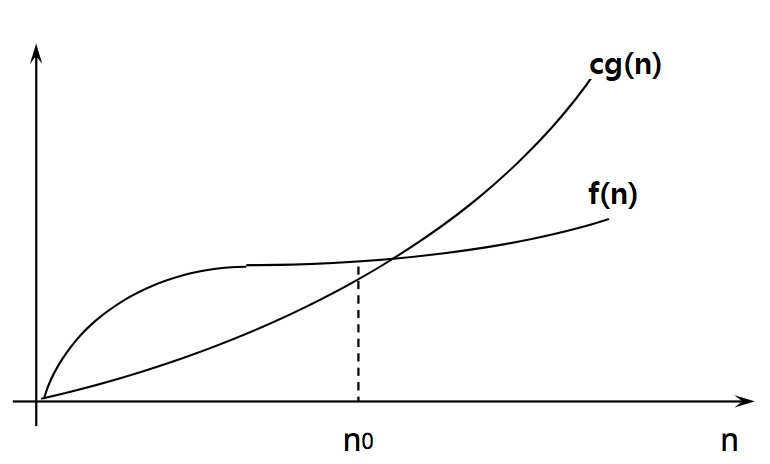
\includegraphics[width=0.7\textwidth]{figures/fig05_bigoh.png}
    \caption{Which one is faster?}
  \end{figure}
\end{frame}

\begin{frame}[t]
  \frametitle{Performance Analysis: Asymptotic Notation}
 f(n) = 25$\cdot$n, g(n) = 1/3$\cdot$n$^2$ 
 %add addional description -2021.01.31 kimsongsub-
\begin{itemize}
\item 25$\cdot$n = O(n$^2$/3) if let c = 1
\item 'f of n' is 'big-oh of g of n'
\end{itemize}

  \begin{figure}[h]
    \centering
    \includegraphics[width=0.5\textwidth]{figures/fig06_accel.png}
    \caption{Which one is faster?}
  \end{figure}
%revised text -2021.01.31 kimsongsub-
$ |25\cdot n|  \leq 1\cdot|n^2/3|$ for all n$ \geq  75$
\end{frame}

\begin{frame}[t]
  \frametitle{Performance Analysis: Asymptotic Notation}
f(n) = O(g(n))
\begin{itemize}
\item g(n) is an upper bound on the value of f(n) for all n, n$\geq$ n0
\item But, doesn’t say anything about how good this bound is
  \begin{itemize}
  \item n = O(n$^2$), n = O(n$^{2.5}$)
  \item n = O(n$^3$), n = O(2$^n$)
  \end{itemize}

\item g(n) should be as small a function
  of n as one can come up with for which f(n) = O(g(n))
\end{itemize}
%add addional description -2021.01.31 kimsongsub-
\textbf{f(n) = O(g(n)) $\neq$  O(g(n)) = f(n)}

(It is meaningless to say that O(g(n)) = f(n) )
\end{frame}

\begin{frame}[t]
  \frametitle{Performance Analysis: Asymptotic Notation}
\textbf{Theorem)} if $f(n) = a_{m}n^m + ... + a_1n + a_0$, then $f(n) = O(n^m)$

\textbf{Proof)}
\begin{align*}
f(n) &\leq  |a_k|·n^k + |a_{k-1}|·n^{k-1} +...+ |a_1|\cdot n + |a_0| \\
& = {|a_k| + |a_{k-1}|/n +...+ |a_1|/n^{k-1}+ |a_0|/n^k}\cdot n^k \\
& \leq  {|a_k| + |a_{k-1}| +...+ |a_1| + |a_0|}\cdot n^k \\
& = c\cdot n^k (c = |a_k|+|a_{k-1}|+...+|a_1|+|a_0|) = O(n^k)
\end{align*}
\end{frame}
%add page and graph -2021.01.31 kimsongsub-
\begin{frame}[t]
	\frametitle{Performance Analysis: Asymptotic Notation}
	\textbf{Omega}
	\textbf{def)} f(n) = $\Omega$ (g(n))
	\begin{itemize}
		\item iff there exist positive constants c and n0 such that f(n)
		c$\cdot$ g(n) for all n, n$\geq$ $n^0$
	\end{itemize}
	\begin{figure}[h]
		\centering
		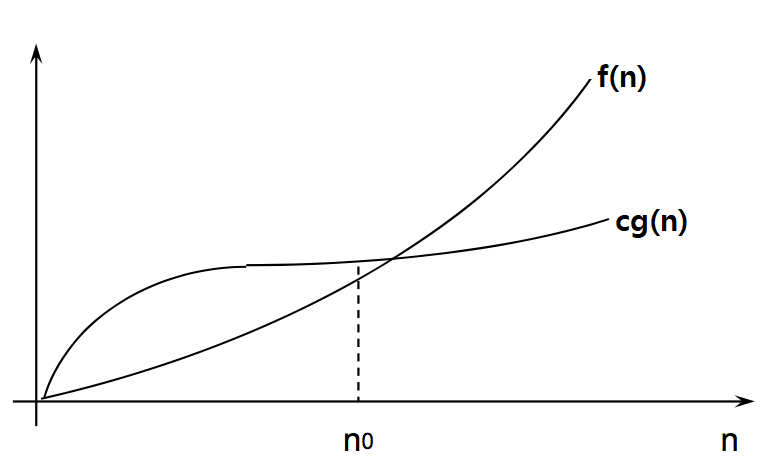
\includegraphics[width=0.7\textwidth]{figures/fig05_omega.png}
		\caption{Which one is faster?}
	\end{figure}
\end{frame}

\begin{frame}[t]
  \frametitle{Performance Analysis: Asymptotic Notation}
  \textbf{Omega}
\begin{itemize}
\item g(n) is a lower bound on the value of f(n) for all n, n $\geq$ n0
\item Should be as large a function of n as possible
\end{itemize}
\textbf{Theorem)} if $f(n) = a_mn^m + ... + a_1n + a_0$ and $am > 0$, then $f(n) = \Omega(n^m)$
\end{frame}
%add page and graph -2021.01.31 kimsongsub-
\begin{frame}[t]
  \frametitle{Performance Analysis: Asymptotic Notation}
\textbf{Theta}
\textbf{def)} f(n) =  $\Theta$(g(n))
\begin{itemize}
\item iff there exist positive constants $c^1$, $c^2$, and $n^0$ such that
\item $c^1\cdot g(n) \leq f(n) \leq c^2\cdot g(n)$ for all n, $n\geq n^0$
\end{itemize}
\begin{figure}[h]
	\centering
	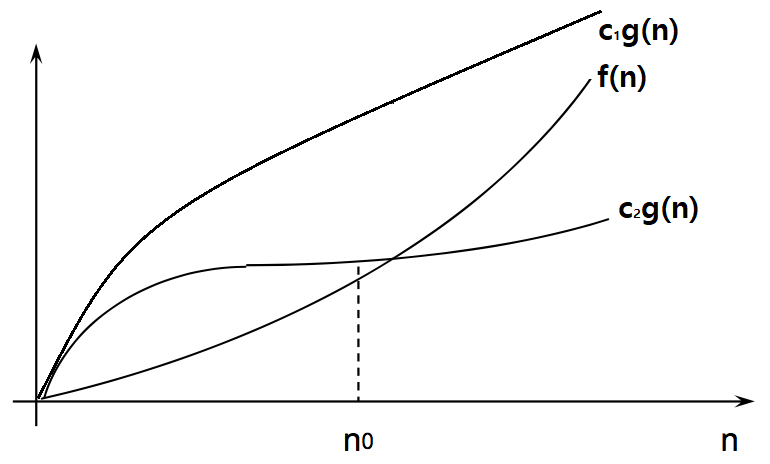
\includegraphics[width=0.7\textwidth]{figures/fig05_theta.png}
	\caption{Which one is faster?}
\end{figure}

\end{frame}

\begin{frame}[t]
	\frametitle{Performance Analysis: Asymptotic Notation}
	\textbf{  Theta}	
	\begin{itemize}
		\item More precise than both the “big oh” and omega notations
		\item g(n) is both an upper and lower bound on f(n)
	\end{itemize}
	
\end{frame}

\begin{frame}[t]
  \frametitle{Performance Analysis: Asymptotic Notation}
Complexity of matrix addition
  \begin{figure}[h]
    \centering
    \includegraphics[width=0.7\textwidth]{figures/fig07_complexity.png}
    \caption{time complexity of matrix addition}
  \end{figure}
\end{frame}

\subsection{Practical Complexities}
\begin{frame}[t]
  \frametitle{Performance Analysis: Practical Complexities}

  \begin{figure}[h]
    \centering
    \includegraphics[width=0.7\textwidth]{figures/fig08_class.png}
    \caption{Class of time complexities}
  \end{figure}
\end{frame}


\begin{frame}[t]
  \frametitle{Performance Analysis: Practical Complexities}
Polynomial time
\begin{itemize}
\item Tractable problem exponential time
\item Intractable (hard) problem
\end{itemize}

Eg)
\begin{itemize}
\item Sequential search
\item Binary search
\item Insertion sort
\item Heap sort
\item Satisfiablity problem
\item Testing serializable scheduling
\end{itemize}

\end{frame}



\begin{frame}[t]
  \frametitle{Performance Analysis: Practical Complexities}

  \begin{figure}[h]
    \centering
    \includegraphics[width=0.9\textwidth]{figures/fig09_func.png}
    \caption{function value}
  \end{figure}
\end{frame}


\begin{frame}[t]
  \frametitle{Performance Analysis: Practical Complexities}

If a program needs $2^n$ steps for execution
\begin{itemize}
\item n=40: number of steps = 1.1*1012 in computer systems
  \begin{itemize}
  \item 1 billion steps/sec --- 18.3 min
  \end{itemize}
\item n=50 --- 13 days
\item n=60 --- 310.56 years
\item n=100 --- 4*1013 years
\end{itemize}

If a program needs $n^{10}$ steps for execution
\begin{itemize}
\item n=10 --- 10 sec
\item n=100 --- 3171 years
\end{itemize}

\end{frame}



\end{document}
